%%%%%%%%%%%%%%%%%%%%%%%%%%%%%%%%%%%%%%%%%%%%%%%%%%%%%%%%%%%%%%%%%%%%%
%% This is a (brief) model paper using the achemso class
%% The document class accepts keyval options, which should include
%% the target journal and optionally the manuscript type. 
%%%%%%%%%%%%%%%%%%%%%%%%%%%%%%%%%%%%%%%%%%%%%%%%%%%%%%%%%%%%%%%%%%%%%
\documentclass[journal=jctcce,manuscript=article]{achemso}
%\documentclass[12pt]{article}
%\usepackage[letterpaper,left=0.5in,right=0.5in,top=1.0in,bottom=1.0in]{geometry}

%%%%%%%%%%%%%%%%%%%%%%%%%%%%%%%%%%%%%%%%%%%%%%%%%%%%%%%%%%%%%%%%%%%%%
%% Place any additional packages needed here.  Only include packages
%% which are essential, to avoid problems later. Do NOT use any
%% packages which require e-TeX (for example etoolbox): the e-TeX
%% extensions are not currently available on the ACS conversion
%% servers.
%%%%%%%%%%%%%%%%%%%%%%%%%%%%%%%%%%%%%%%%%%%%%%%%%%%%%%%%%%%%%%%%%%%%%
\usepackage[version=3]{mhchem} % Formula subscripts using \ce{}
\usepackage{siunitx} % generating degrees Celsius in the document 
\usepackage{color}
\usepackage{soul} % allows highlighting text 
\usepackage{makecell}
\usepackage{booktabs}



%%%%%%%%%%%%%%%%%%%%%%%%%%%%%%%%%%%%%%%%%%%%%%%%%%%%%%%%%%%%%%%%%%%%%
%% If issues arise when submitting your manuscript, you may want to
%% un-comment the next line.  This provides information on the
%% version of every file you have used.
%%%%%%%%%%%%%%%%%%%%%%%%%%%%%%%%%%%%%%%%%%%%%%%%%%%%%%%%%%%%%%%%%%%%%
%%\listfiles

%%%%%%%%%%%%%%%%%%%%%%%%%%%%%%%%%%%%%%%%%%%%%%%%%%%%%%%%%%%%%%%%%%%%%
%% Place any additional macros here.  Please use \newcommand* where
%% possible, and avoid layout-changing macros (which are not used
%% when typesetting).
%%%%%%%%%%%%%%%%%%%%%%%%%%%%%%%%%%%%%%%%%%%%%%%%%%%%%%%%%%%%%%%%%%%%%
\newcommand*\mycommand[1]{\texttt{\emph{#1}}}

%%%%%%%%%%%%%%%%%%%%%%%%%%%%%%%%%%%%%%%%%%%%%%%%%%%%%%%%%%%%%%%%%%%%%
%% Meta-data block
%% ---------------
%% Each author should be given as a separate \author command.
%%
%% Corresponding authors should have an e-mail given after the author
%% name as an \email command. Phone and fax numbers can be given
%% using \phone and \fax, respectively; this information is optional.
%%
%% The affiliation of authors is given after the authors; each
%% \affiliation command applies to all preceding authors not already
%% assigned an affiliation.
%%
%% The affiliation takes an option argument for the short name.  This
%% will typically be something like "University of Somewhere".
%%
%% The \altaffiliation macro should be used for new address, etc.
%% On the other hand, \alsoaffiliation is used on a per author basis
%% when authors are associated with multiple institutions.
%%%%%%%%%%%%%%%%%%%%%%%%%%%%%%%%%%%%%%%%%%%%%%%%%%%%%%%%%%%%%%%%%%%%%
\author{Stephen P. Vicchio}
\affiliation[Clemson University]
{Department of Chemical and Biomolecular Engineering, Clemson University, Clemson, SC}
\author{Sachi Hilliard}
\affiliation[Clemson University]
{Department of Chemical and Biomolecular Engineering, Clemson University, Clemson, SC}
%\author{Omar Farha?}
%\affiliation[Northwestern University]
%{Northwestern University}
\author{Rachel B. Getman}
\email{rgetman@g.clemson.edu}
\affiliation[Clemson University]
{Department of Chemical and Biomolecular Engineering, Clemson University, Clemson, SC}


%%%%%%%%%%%%%%%%%%%%%%%%%%%%%%%%%%%%%%%%%%%%%%%%%%%%%%%%%%%%%%%%%%%%%
%% The document title should be given as usual. Some journals require
%% a running title from the author: this should be supplied as an
%% optional argument to \title.
%%%%%%%%%%%%%%%%%%%%%%%%%%%%%%%%%%%%%%%%%%%%%%%%%%%%%%%%%%%%%%%%%%%%%
\title[manuscript]{Nickel(II) and Copper(II) Supported Metal Complex Stability in NU-1000 Under Hydrogenation Conditions}

%%%%%%%%%%%%%%%%%%%%%%%%%%%%%%%%%%%%%%%%%%%%%%%%%%%%%%%%%%%%%%%%%%%%%
%% Some journals require a list of abbreviations or keywords to be
%% supplied. These should be set up here, and will be printed after
%% the title and author information, if needed.
%%%%%%%%%%%%%%%%%%%%%%%%%%%%%%%%%%%%%%%%%%%%%%%%%%%%%%%%%%%%%%%%%%%%%
\abbreviations{IR,NMR,UV}
\keywords{American Chemical Society, \LaTeX}

%%%%%%%%%%%%%%%%%%%%%%%%%%%%%%%%%%%%%%%%%%%%%%%%%%%%%%%%%%%%%%%%%%%%%
%% The manuscript does not need to include \maketitle, which is
%% executed automatically.
%%%%%%%%%%%%%%%%%%%%%%%%%%%%%%%%%%%%%%%%%%%%%%%%%%%%%%%%%%%%%%%%%%%%%
\begin{document}

%%%%%%%%%%%%%%%%%%%%%%%%%%%%%%%%%%%%%%%%%%%%%%%%%%%%%%%%%%%%%%%%%%%%%
%% The "tocentry" environment can be used to create an entry for the
%% graphical table of contents. It is given here as some journals
%% require that it is printed as part of the abstract page. It will
%% be automatically moved as appropriate.
%%%%%%%%%%%%%%%%%%%%%%%%%%%%%%%%%%%%%%%%%%%%%%%%%%%%%%%%%%%%%%%%%%%%%
%\begin{tocentry}
%
%Some journals require a graphical entry for the Table of Contents.
%This should be laid out ``print ready'' so that the sizing of the
%text is correct.
%
%Inside the \texttt{tocentry} environment, the font used is %Helvetica
%8\,pt, as required by \emph{Journal of the American Chemical
%Society}.
%
%The surrounding frame is 9\,cm by 3.5\,cm, which is the maximum
%permitted for  \emph{Journal of the American Chemical Society}
%graphical table of content entries. The box will not resize if the
%content is too big: instead it will overflow the edge of the box.
%
%This box and the associated title will always be printed on a
%separate page at the end of the document.
%
%\end{tocentry}

%%%%%%%%%%%%%%%%%%%%%%%%%%%%%%%%%%%%%%%%%%%%%%%%%%%%%%%%%%%%%%%%%%%%%
%% The abstract environment will automatically gobble the contents
%% if an abstract is not used by the target journal.
%%%%%%%%%%%%%%%%%%%%%%%%%%%%%%%%%%%%%%%%%%%%%%%%%%%%%%%%%%%%%%%%%%%%%
\begin{abstract}
    
\end{abstract}

%%%%%%%%%%%%%%%%%%%%%%%%%%%%%%%%%%%%%%%%%%%%%%%%%%%%%%%%%%%%%%%%%%%%%
%% Start the main part of the manuscript here.
%%%%%%%%%%%%%%%%%%%%%%%%%%%%%%%%%%%%%%%%%%%%%%%%%%%%%%%%%%%%%%%%%%%%%
\newpage
\section{Introduction}
%\begin{itemize}
%    \item Goal is to perform energy-efficient GTL conversions using catalysts. 
%    \item Potential solution is supporting metal complexes in MOFs.
%    \begin{itemize}
%        \item What are MOFs? What are they comprised of?
%        \item What are metal complexes? What are some of the advantages and disadvantages? 
%    \end{itemize}
%    \item Highlight some of the previous literature on MOFs as catalyst supports. 
%    \begin{itemize}
%        \item articles on ethylene hydrogenation
%        \item articles on ethylene dimerization 
%        \item article on methane partial oxidation
%        \item articles on oliogermization 
%    \end{itemize}
%    \item \emph{Emphasize the research question: how does the reaction environment influence %the catalyst structure (morphology and composition)?}
%    \begin{itemize}
%        \item The paper from ICDC that discusses Cu NP formation for Cu-NU-1000 %(\citeauthor{Halder2020}).
%        \item The discussion that waters are removed to generate the activated catalyst. 
%        \item What happens when that catalyst is exposed to molecular hydrogen? Could the %stability of the catalyst be compromised?
%    \end{itemize}
%    \item Outcomes of the paper:
%    \begin{itemize}
%        \item Probe catalyst stability in environments containing \ce{H2} for both \ce{Ni} %and \ce{Cu} supported metal complexes as a function of temperature, and \ce{H2} and %\ce{H2O} partial pressures. 
%    \end{itemize}
%\end{itemize}


%\begin{figure}[t]
%    \centering
%    \includegraphics[width=0.95\textwidth]{zi-images/00-General-Graphics/2020-07-31-Combined-%MOF-Figure-final.png}
%    \caption{The structure of NU-1000, which is comprised of (a)  inorganic nodes %(\ce{[Zr6(\mu3-O)4(\mu3-OH)4(H2O)4(OH)4]^8^+}) and (b) organic linkers %(1,3,6,8-tetrakis(p-benzoic acid)pyrene (\ce{TBAPy^4^-})) to produce (c) the framework %structure (with the c-pore highlighted by the gray box). Additionally, the two metal %complexes supported in the c-pore of NU-1000 are also shown: (d) the \ce{Cu3(OH)4} metal %complex, and (d) the \ce{Ni4(OH)6} metal complex.}
%    \label{fig:MOFstructure}
%\end{figure}


\begin{enumerate}
    \item Paragraph 1: General introduction about these catalysts.
    \begin{itemize}
        \item General discussion about MOFs as catalyst supports and the creation of catalysts from metal complexes. 
    \end{itemize}
    \item Paragraph 2: More information about the metal complexes supported on NU-1000. 
    \begin{itemize}
        \item The different types of supported metal complexes (\ce{Ni(II)}, \ce{Cu(II)}, etc/.) and how they are attached to the node. 
        \item Are they attached to a single node in the MOF framework? Are they attached to multiple nodes in the framework? 
    \end{itemize}
    \item Paragraph 3: Limitations of not knowing the exact active site. 
    \begin{itemize}
        \item Emphasize the research question: how does the reaction environment influence the catalyst structure (morphology and composition)?
        \item To understand the catalysis, we need an understanding of the active site. The structure of the active site will determine the function of the catalyst.
        \item Talk about the original paper from Jingyun about looking at \ce{Ni1} vs. 
        \ce{Ni4} clusters and 
        \item Talk about Hafeera's work on hydrogenation and how some of the metal trends agree whereas others do not.. and suggest that maybe these differences could be attributed to incorrect models? Rather then all being single metal sites, maybe some of those metal sites were multiple atoms? Could the conditions explain that? 
        \item Talk the papers (Halder, Jingyun \ce{Cu} clusters, \ce{Ni4} proposed cluster) that discuss the dynamic changes these clusters exhibit to add emphasis in how important it is to understand the active site (not on when synthesized, but also under reaction conditions). 
    \end{itemize}
    \item Paragraph 4: Summary of current findings. 
    \begin{itemize}
        \item \ce{Ni} does not completely reduce to form NPs. \ce{Ni} cluster changes via removal of \ce{OH} ligands as \ce{H2O}, but the Ni atoms remain attached to the cluster. The presence of \ce{Ni-H} is captured in the modeling analysis. 
        \item \ce{Cu(II)} cluster completed reduces and is stripped away from the cluster. Intermediate structures suggest the presence of \ce{Cu-H} structures. 
    \end{itemize}
\end{enumerate}

% The introduction section should consist of 4 paragraphs. 

% Paragraph 1: General Statement about these catalysts 


% Paragraph 2: More specific issue and problems 
% the different types of potential models for these systems.. there are different modeling choices that can be made for these systems.. talk about the different Ni(II) models comprised of a single Ni(II) atoms.. 


% Paragraph 3: 
% Talk about some of the limitations.. if we want to model the catalysis, we need a reasonable structures to determine the kinetic information.. we don't have that information.. we are missing out on appropriate models.. numerous papers that suggest that modeling is appropriate.. however,. what about the differences in trends between different models..? That could be a major issue and something worth thinking about more.. 



% Paragraph 4: specifically what has been shown for your work (think precursor here for your project
% here I state specifically what I find in my paper..


% think back to the discuss that I had with Rachel about the paper.. that's what she wants me to include for this section.. I need to talk and emphasize the catalyst structure here, which is something that needs to be done... I can do that.. for sure.. I just need to spend the time in trying to write up that section for this particular paper --> really focus on what those reference structure are going to be actually be like here. 

%%%%%%%%%%%%%%%%%%%%%%%%%%%%%%%%%%%%%%%%%%%%%%%%%%%%%%%%%%%%%%%%%%%%%
%% Methodology
%%%%%%%%%%%%%%%%%%%%%%%%%%%%%%%%%%%%%%%%%%%%%%%%%%%%%%%%%%%%%%%%%%%%%

\newpage
\section{Methodology}
%To capture how the supported metal complex  (structure and composition) is impacted by the %reaction conditions (temperature ($T$), pressure ($P$), and composition), \textit{ab initio} %thermodynamic analysis was used.\textit{ab initio} thermodynamic analysis, also called %"first-principles thermodynamics," has been used to study the influence of gas phase conditions %on catalysis on Oxygen Chemisorption on \ce{Pt(111)},\cite{Getman2008} the interactions between %cluster-support and cluster-adsorbate \ce{Pt8} clusters on alumina in a hydrogen gas (\ce{H2}) %environment,\cite{Sun2019} and the structure and reversibility of \ce{Cu}-oxo active %sites.\cite{Grundner2015,Li2016,Paolucci2016} The stability of two metal complexes (Cu-NU-1000 %and Ni-NU-1000) in a reducing environment were investigated.  
%
%To determine the relative stability of different activated Cu-NU-1000 and Ni-NU-1000, the %following reversible reaction was constructed  to compare structures with different chemical %compositions: 
%\begin{equation} \label{exp:gibbsfreeoverall}
%    \ce{z * H2 (g) + Cu3(OH)4-MOF <=>[$\Delta G(T,P)$] Cu3O_{4-n}H_{4+2z-2n}-MOF + n * H2O}
%\end{equation}
%where \ce{z} is the number of molecular \ce{H2} that are dissociatively adsorbed onto the %activated cluster supported on the NU-1000 MOF (\ce{Cu3(OH)4-MOF}), \ce{n} is the number %\ce{OH}-ligands that are converted into \ce{H2O} that are removed from the starting cluster, %and \ce{Cu3O_{4-n}H_{4+2z-2n}-MOF} cluster, and $\Delta G(T,P)$ is the equilibrium Gibbs free %energy at a specific temperature ($T$) and pressure ($P$). The reference state for all %calculations is the experimentally synthesized structure (Figure \ref{fig:MOFstructure} e) and %d)), meaning in the absences of \ce{H2} gas the cluster will remain as the experimentally %synthesized structure comprised of metal hydroxo clusters. The equilibrium Gibbs free energy %for Equilibrium \ref{exp:gibbsfreeoverall} can be written as:
%\begin{equation} \label{eqn:gen-ab-initio}
%    \begin{split}
%        \Delta G(T,P) & = \Delta G_{\ce{Cu3O_{4-n}H_{4+2z-2n}-MOF}} + n \cdot %\mu_{H_{2}O}^{*}(T,P) - \Delta G_{\ce{Cu3(OH)4-MOF}} - 2 \cdot z \cdot \mu_{H}^{*}(T,P)
%    \end{split}
%\end{equation}
%where $\Delta G_{\ce{Cu3O_{4-n}H_{4+2z-2n}-MOF}}$ is the Gibbs free energy of the activated %species, $\Delta G_{\ce{Cu3(OH)4-MOF}}$ is the Gibbs free energy of the starting cluster, %$\mu_{H_{2}O}^{*}$ is the chemical potential of \ce{H2O} adsorbed species, and $\mu_{H}^{*}$ is %the chemical potential of an adsorbed \ce{H} atom. Analogous expressions for and Equation %\ref{eqn:gen-ab-initio} where also created for the \ce{Ni4(OH)6} cluster (see \hl{Supporting %Information)}. 
%
%In Equation \ref{eqn:gen-ab-initio}, the vibrational and pressure-volume contributions to the %Gibbs free energy were neglected for the cluster structures (\ce{Cu3(OH)4-MOF} and %\ce{Cu3O_{4-n}H_{4+2z-2n}-MOF}), allowing the Gibbs free energies to be approximated by their %electronic energies computed with Density Functional Theory (DFT). The chemical potential %terms, $\mu_{H}^{*}$ and $\mu_{H_{2}O}^{*}$, are dependent on the gas phase conditions ($T$ and %$P$). The adsorbed species, \ce{H2O} and \ce{H2}, are assumed to form an ideal-gas-like %reservoir with $\mu_{H}^{g}$ and $\mu_{H_{2}O}^{g}$, respectively. Therefore, the following %equilibrium expression and chemical reaction and were written:   
%\begin{equation} \label{exp:chemicalpotential}
%    \ce{1/2 H2(g) <=> $\mu_{H}^{*}$}
%\end{equation}
%\begin{equation} \label{eqn:chemicalpotential}
%    \frac{1}{2} \: \mu_{H}^{g}(T,P) = \mu_{H}^{*}(T,P)
%\end{equation}
%where $\mu_{H}^{g}$ is the gas phase chemical potential. The gas chemical potential terms were %computed by correcting the electronic energy (referenced at $T$=0 K) of an isolated molecule %with the gas-phase Gibbs free energy values. The gas-phase Gibbs free energies were computed %using the NASA Polynomials\cite{Mcbride1993} using pMuTT.\cite{LYM2019106864} The previous %assumption allow the chemical potential (as a function of $T$ and $P$) to be written as %follows:  
%\begin{equation}
%     \mu_{H}^{g}(T,P) = \frac{1}{2} E_{H_2} + \Delta \mu_{H}(T,P)
%\end{equation}
%where
%\begin{equation}
%    \begin{split}
%    \Delta \mu_{H}(T,P) 
%    & = \Delta \mu_{H}(T,P^{0}) + \frac{1}{2} RT \ln{(\frac{P_{H_{2}}}{P_{H_{2}}^{0}})} \\
%    & = \frac{1}{2} \Delta \mu_{H_{2}}(T,P^{0}) + \frac{1}{2} RT %\ln{(\frac{P_{H_{2}}}{P_{H_{2}}^{0}})} \\
%    & = \frac{1}{2} \bigg[ \Delta G_{H_{2}}(T,P^{0}) + RT %\ln{(\frac{P_{H_{2}}}{P_{H_{2}}^{0}})} \bigg] \\  
%    & = \frac{1}{2} \bigg[G_{H_{2}}(T,P^{0}) - G_{H_{2}}(0\;K,P^{0}) + RT %\ln{(\frac{P_{H_{2}}}{P_{H_{2}}^{0}})} \bigg]
%    \end{split}
%\end{equation}
%The gas phase values provided by pMuTT are referenced at $T=$ \SI{298}{Kelvin}; therefore, the %gas phase Gibbs Free energy were converted to be referenced at $T=$ \SI{10}{Kelvin} (see the %\hl{Supporting Information} for more details). An analogous expression was constructed for %\ce{H2O} (see \hl{Supporting Information}) to relate the gas phase Gibbs Free energy of %\ce{H2O} to the $\mu_{H_{2}O}^{*}$ chemical potential term. The electronic energies were again %calculated using DFT.  
%
%All electronic energies were computed from periodic density functional calculations in %CP2K.\cite{Hutter2014} The exchange correlation energy was calculated with the PBE %functional\cite{Perdew1996} and corrected using damped D3 dispersion corrections formulated by %\citeauthor{Grimme2010}.\cite{Grimme2010} The DZVP-MOLOPT basis set (\hl{reference}) was used %to describe the valance electrons, Goedecker pseudopotentials\cite{Goedecker1996} to describe %the core electron, and a plane wave cutoff energy of 360 Ry. All atoms in the periodic unit %cell were allowed to relax during geometry optimizations. For each activated cluster, the %computed electronic energies terms were input into Equation \ref{eqn:gen-ab-initio}. By varying %the chemical potentials terms for both \hl{$\mu_{H2O}$ and $\mu_{H2}$}, the $\Delta %G(T,P,\mu_{H2O},\mu_{H2})$ was determined for a range of reaction conditions. Identifying the %lowest $\Delta G(T,P,\mu_{H_{2}O},\mu_{H_{2}})$ for all activated clusters revealed the most %favorable structure under those conditions.


% The new updated methodology section based on Rachel's suggestions and recommendations: 

% (1) define the reference MOF structure as the starting structure in my analysis and the modified structure as.. write the expressions in terms of a generalized approach here.  
We demonstrate the influence of reaction conditions, such as temperature ($T$) and pressure ($P$), on supported metal complex stability using thermodynamic analysis to compute the free energy of different activated structures. Specifically, \textit{ab initio} thermodynamic analysis computes the structurally stability of compositionally different structures by transforming the free energy from a fixed number of atoms to a fixed chemical potential. The reference supported metal complex on NU-1000, formed from the ALD process, is comprised of adsorbed \ce{OH^{*}} and \ce{M^{*}} species and is activated with molecular \ce{H2} to form \ce{H^{*}} species. The \ce{H^{*}} species are attached to either the \ce{OH^{*}} species forming waters (\ce{H2O^{*}}) or the \ce{M^{*}} species forming metal hydrides (\ce{M-H}). The newly formed modified structure exhibits different composition of \ce{H^{*}}, \ce{OH^{*}} and \ce{M^{*}} species compared to the reference structure. We generate a library of unique, candidate modified structures for the \textit{ab initio} thermodynamic analysis by systematically adding \ce{H} atoms to different atoms on metal cluster and removing any formed \ce{H2O} (\hl{see Supporting Information for further details}).

By transforming the free energy from a fixed number of atoms to a fixed chemical potential ($\mu_{H^{*}}$, $\mu_{OH^{*}}$, and $\mu_{Ni^{*}}$), we determine the thermodynamically favorable modified structures despite having different compositions. Equation \ref{eq:free-energy-trans} shows the generalized free energy expression \hl{(see Supporting Information for more information on derivation).}
\begin{equation}
    \begin{split}
        \Delta G^{(3)}(T,\mu_{H^{*}},\mu_{OH^{*}},\mu_{M^{*}})  = & \Delta G(T,N_{H^{*}},N_{OH^{*}},N_{Ni^{*}}) - (\mu_{H^{*}})(\Delta N_{H^{*}}) \\
        & - (\mu_{OH^{*}})(\Delta N_{OH^{*}}) 
          - (\mu_{M^{*}})(\Delta N_{M^{*}}) \\ 
    \end{split}
    \label{eq:free-energy-trans}
\end{equation}
The $\Delta G(T,N_{H^{*}},N_{OH^{*}},N_{Ni^{*}})$ term is the difference in the modified structure and reference structure (defined here as the as-synthesized, starting MOF structure). The chemical potential terms,  $\mu_{H^{*}}$ and $\mu_{OH^{*}}$, depend on the temperature and gas phase reaction conditions because we assume that the adsorbate species are in equilibrium with an ideal-gas like reservoir with \ce{H2} and \ce{H2O} species. The chemical potential of the reservoir is dependent on the reaction conditions. 

At equilibrium, the chemical potential of the adsorbate species is equal to the chemical potential of the gas phase species. The assumed equilibrium for $\ce{H^{*}}$ is with $\frac{1}{2}\ce{H_{2}^{g}}$ and for $\ce{OH^{*}}$ is with $\ce{H_{2}O^{g}}$/$\frac{1}{2}\ce{H_{2}^{g}}$. The combined expression for $\ce{OH^{*}}$ captures the influence of both \ce{H2O} and \ce{H2} gas phase conditions on the stability of the cluster. For further details \hl{see Support Information}. The metal chemical potential term ($\mu_{M^{*}}$) is independent of the reaction conditions and the metal chemical potential term is approximated by free energy for a bulk metal system. Equation \ref{eq:chemicalpotentialeq} shows the chemical potential expressions for the $\ce{H^{*}}$ and $\ce{OH^{*}}$ adsorbed species with respect to gas phase \ce{H2} and \ce{H2O} conditions. \begin{equation}
    \begin{split}
        \mu_{H^{*}} &= \frac{1}{2} \mu_{H_{2}}^{g}(T,P) \\ 
        \mu_{OH^{*}} &= \mu_{H_{2}O}^{g}(T,P) - \frac{1}{2} \mu_{H_{2}}^{g}(T,P) \\
    \end{split}
    \label{eq:chemicalpotentialeq}
\end{equation}
The $\mu_{i}^{g}(T,P)$ terms contain the temperature and pressure influences of the reaction conditions.\textit{ab initio} thermodynamic analysis determines the thermodynamically stable structures by computing the free energy (Equation \ref{eq:free-energy-trans}) as a function of gas phase chemical potential species for all structures in the library. At every combination of $\mu_{H_{2}}^{g}(T,P)$ and $\mu_{H_{2}O}^{g}(T,P)$, the structure with the lowest free energy is identified to generate phase diagrams revealing the thermodynamic landscape of the modified metal cluster under reducing conditions. 

The gas phase chemical potential terms ($\mu_{i}^{g}(T,P)$) are computed by by correcting the electronic energy (referenced at $T$=0 K) of an isolated molecule with the gas-phase Gibbs free energy values at a specific temperature and pressure (Equation \ref{eq:chemicalpotentialrel}).
\begin{equation}
    \begin{split}
        \mu_{H_{2}}^{g}(T,P) &= E_{H_2} + \Delta \mu_{H_{2}}(T,P)  = E_{H_{2}} + \Big[ \Delta G_{H_{2}}(T,P^{o}) + RT \ln{\Big( \frac{P_{H_{2}}}{P^{o}} \Big)} \Big] \\  
        \mu_{H_{2}O}^{g}(T,P) &= E_{H_{2}O} + \Delta \mu_{H_{2}O}(T,P^{o}) =  E_{H_{2}O} + \Big[ \Delta G_{H_{2}O}(T,P^{o}) + RT \ln{\Big( \frac{P_{H_{2}O}}{P^{o}} \Big)} \Big]
    \end{split}
    \label{eq:chemicalpotentialrel}
\end{equation}
 The gas-phase Gibbs free energies ($\Delta G_{i}(T,P^{o})$) were computed using the NASA Polynomials\cite{Mcbride1993} in the pMuTT\cite{LYM2019106864} Python package at standard pressure ($P^{o}$) to capture the influence of temperature. The pressure effects are captured assuming ideal gas for the gas phase species. 
 
All electronic energies were computed from periodic density functional calculations in CP2K.\cite{Hutter2014} The exchange correlation energy was calculated with the PBE functional\cite{Perdew1996} and corrected using damped D3 dispersion corrections formulated by \citeauthor{Grimme2010}.\cite{Grimme2010} The DZVP-MOLOPT basis set (\hl{reference}) describes the valance electrons, Goedecker pseudopotentials\cite{Goedecker1996} describes the core electron. The plane wave cutoff energy is 360 Ry and  all atoms in the periodic unit cell were allowed to relax during geometry optimizations.

Unrestricted Kohn-Sham (UKS) is implemented because of the variable spin states of metal atoms. For example, \ce{Ni(II)} can adopt both singlet (no unpaired electrons) and triplet (two unpaired electron) configurations. For clusters compromised of multiple metal atoms, all permutations of spin state configurations are simulated. Any structures exhibiting spin contamination were removed from the analysis \hl{see support information for more details}.   


%%%%%%%%%%%%%%%%%%%%%%%%%%%%%%%%%%%%%%%%%%%%%%%%%%%%%%%%%%%%%%%%%%%%%
%% Results
%%%%%%%%%%%%%%%%%%%%%%%%%%%%%%%%%%%%%%%%%%%%%%%%%%%%%%%%%%%%%%%%%%%%%
\newpage
\section{Results}
\subsection{Cu-NU-1000}

\begin{figure}[H]
    \centering
    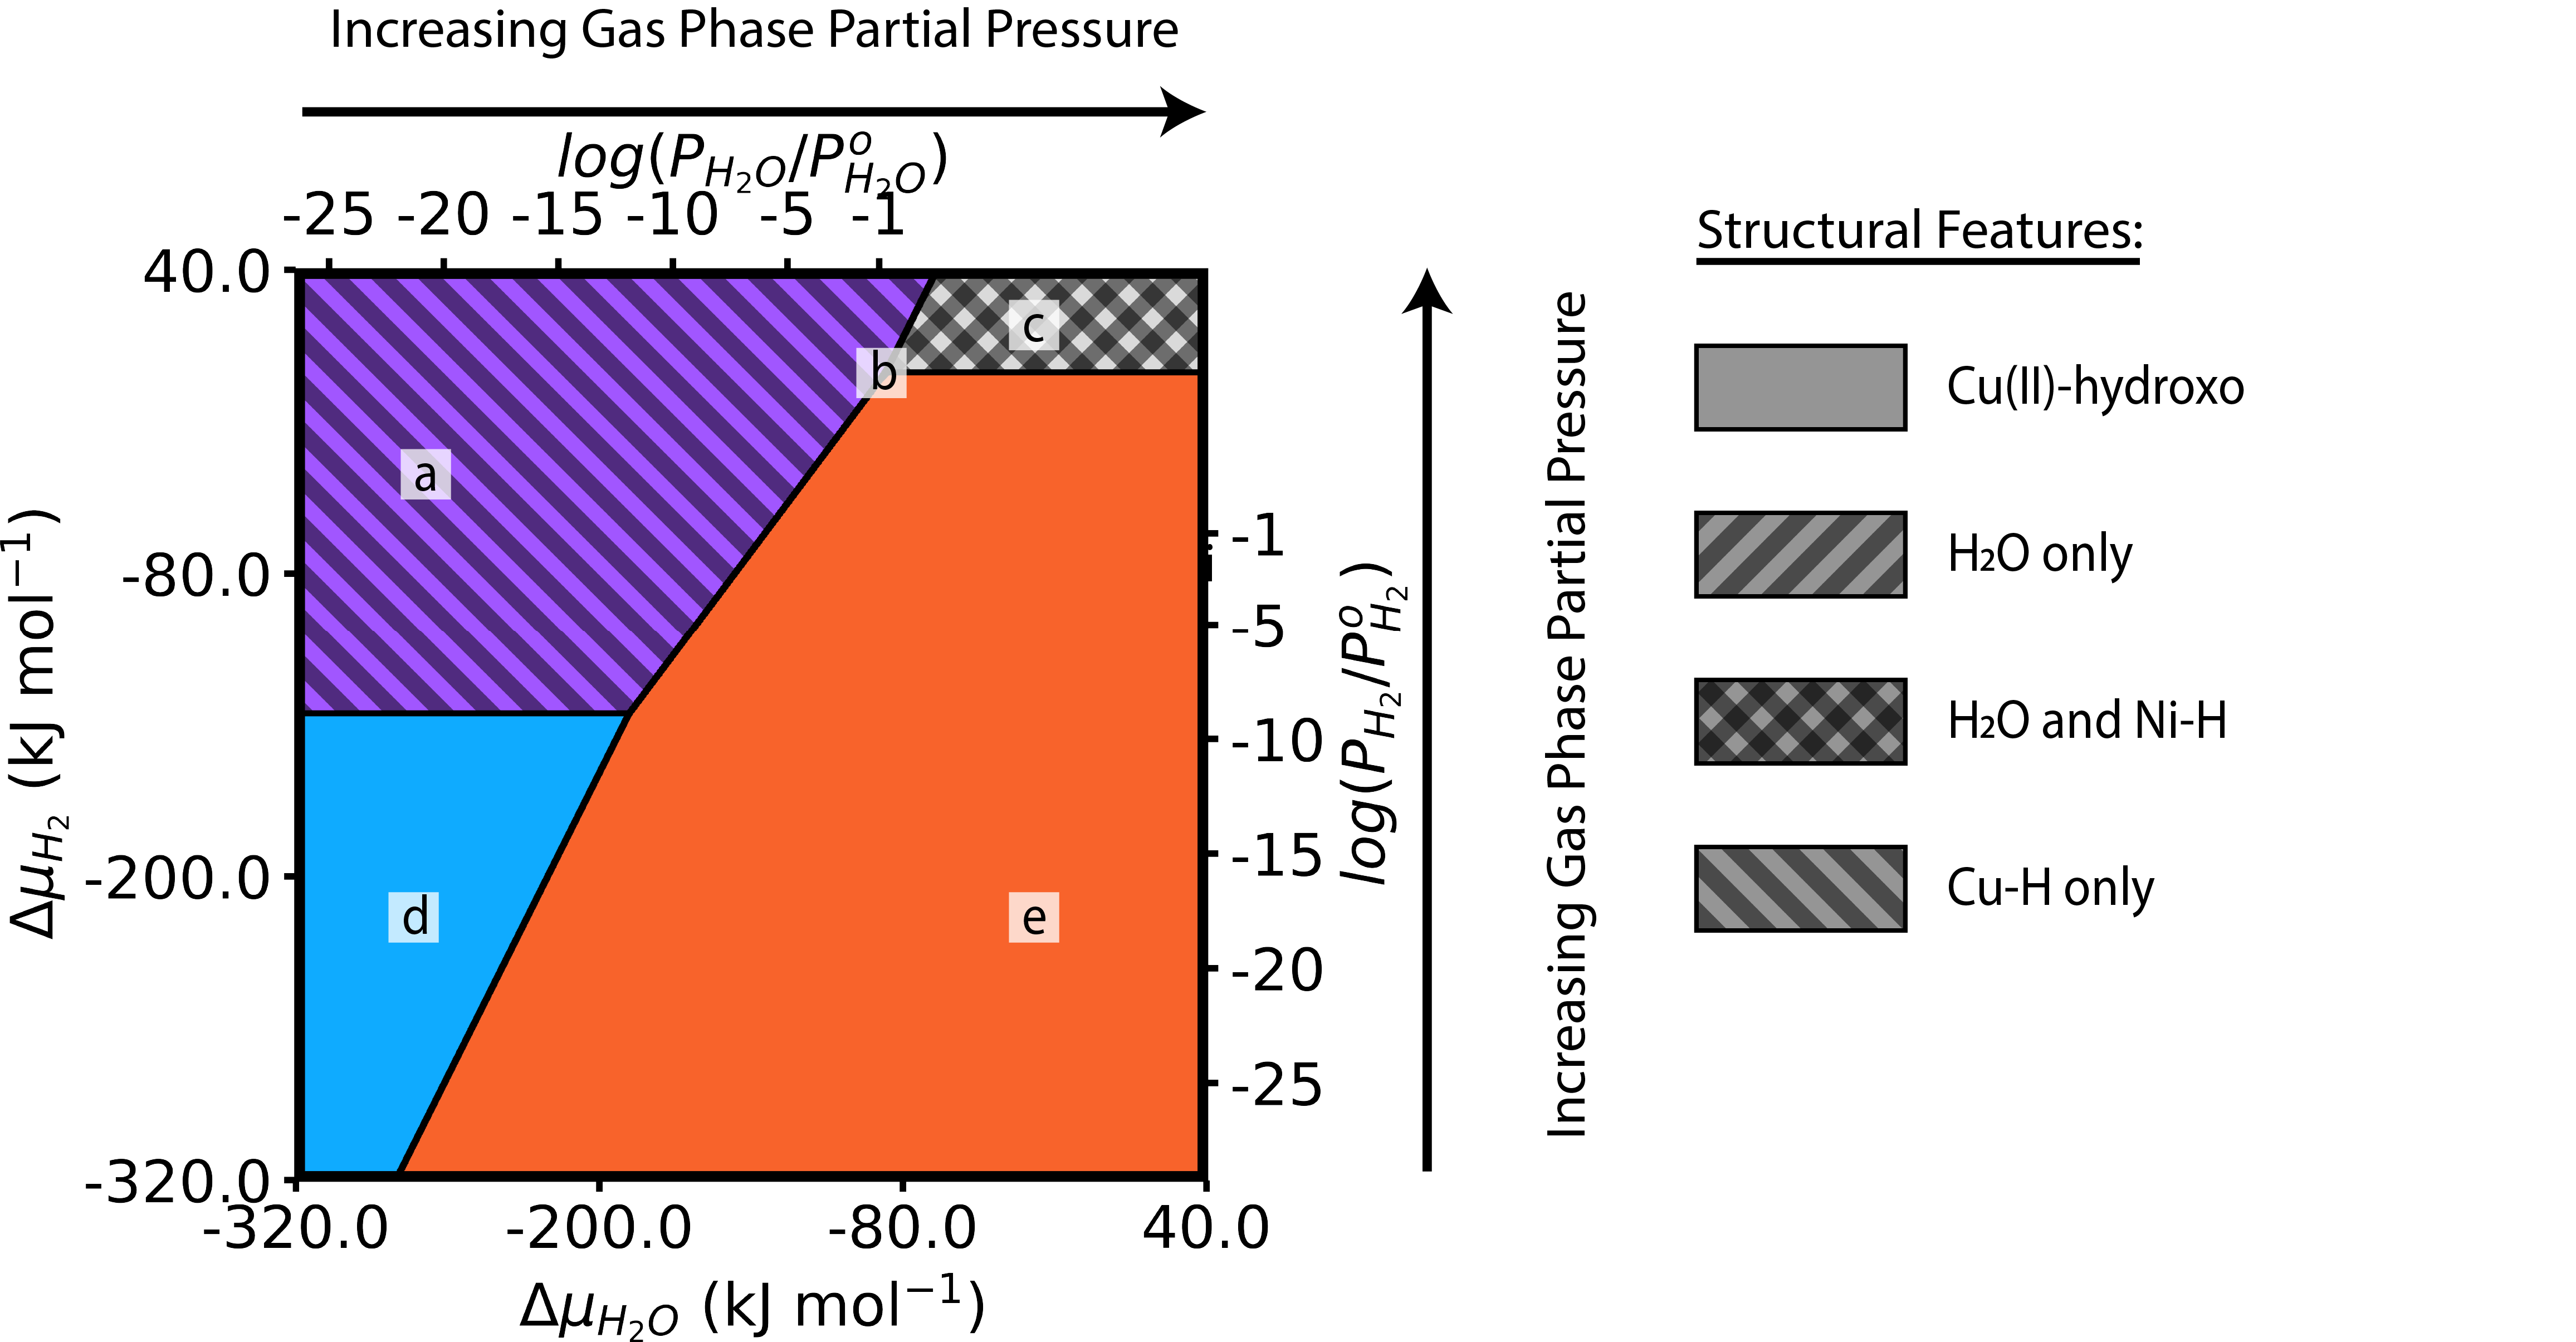
\includegraphics[width=0.95\textwidth]{zi-images/02-Cu-Graphics/2020-08-05-Cu3-phase-diagram-V01.png}
    \caption{Phase diagram generate by \textit{ab initio} thermodynamic analysis that captures the structural stability of a Cu(II) supported metal complex in NU-1000 at \SI{200}{\celsius}. The starting structure is the \ce{Cu3(OH)4} complex. The composition and morphology of the Cu(II) complex changes depending on the \ce{H2} and \ce{H2O} partial pressures, which produces new structural features, such as physisorbed \ce{H2O} and metal hydride structures.}
    \label{fig:phasediagramCu3}
\end{figure}

\begin{figure}[H]
    \centering
    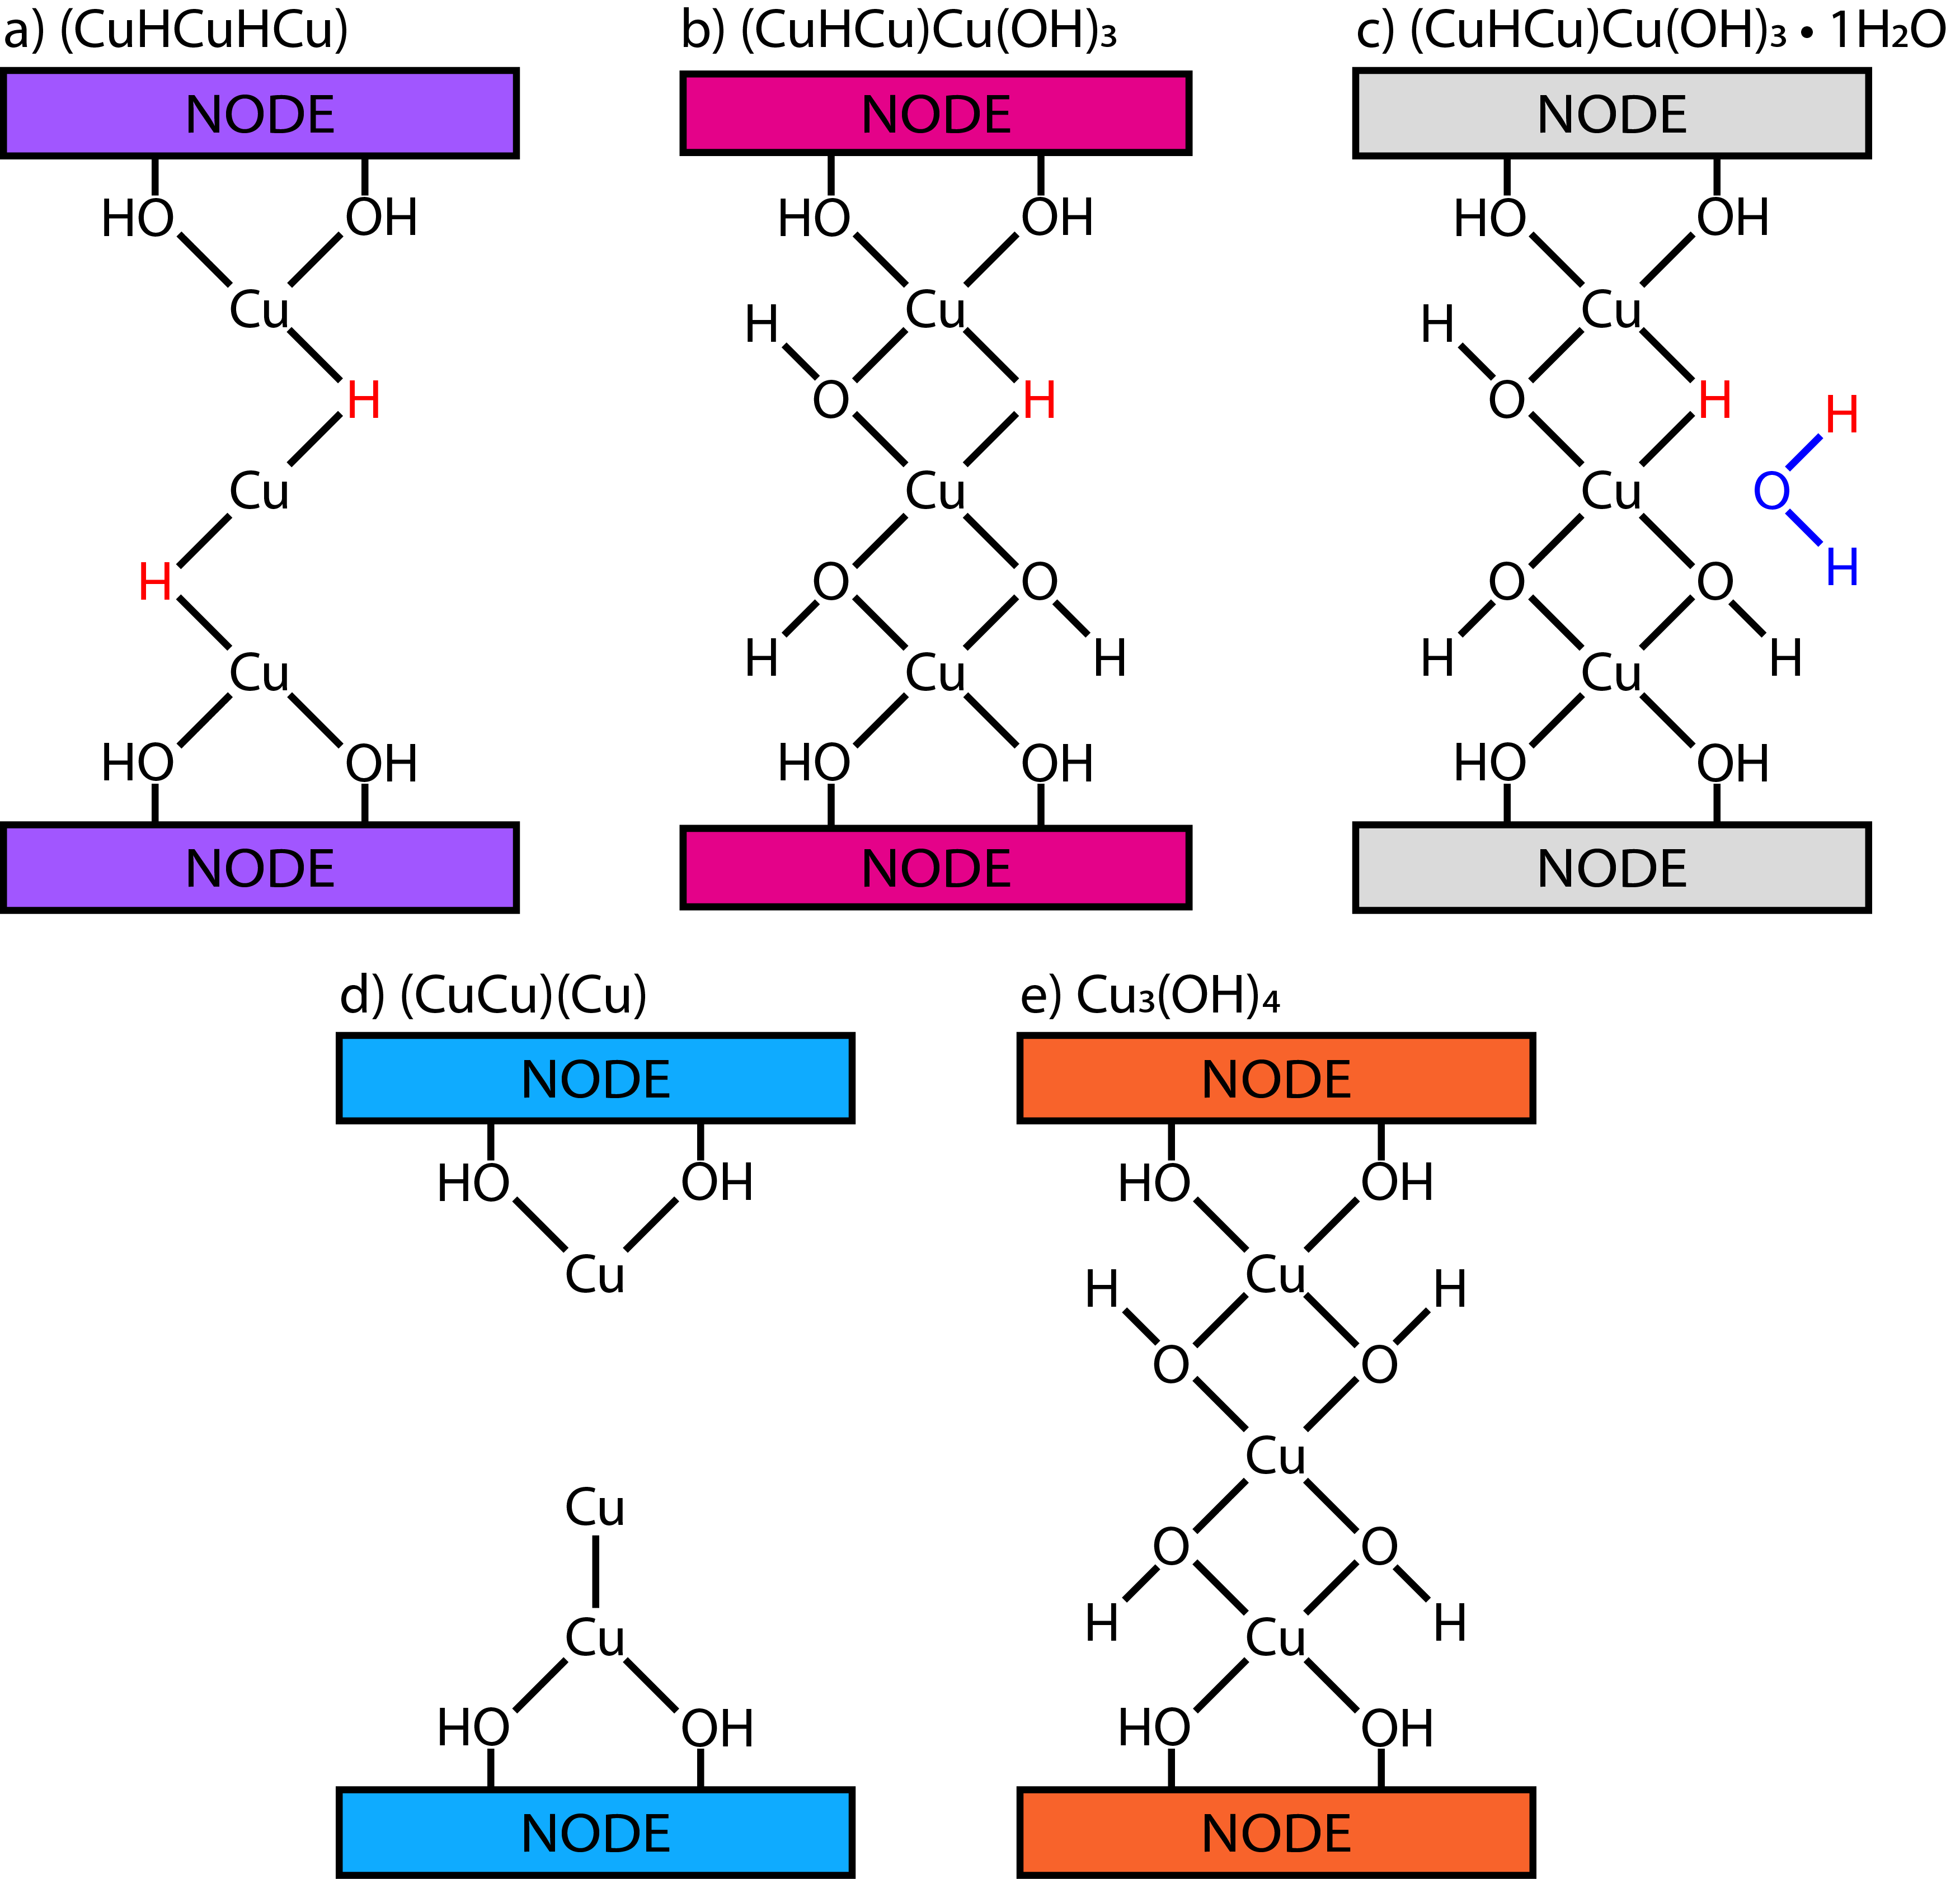
\includegraphics[width=0.85\textwidth]{zi-images/02-Cu-Graphics/2020-08-04-structure-diagram-Cu3OH4-V01-IMAGE.png}
    \caption{Schematic representation of the lowest energy structures from the \textit{ab initio} thermodynamic analysis. The node colors scheme correspond to the \ce{Cu(II)} supported metal complex phase diagram (Figure \ref{fig:phasediagramCu3}).}
    \label{fig:structurediagramCu3}
\end{figure}

\begin{center}
\begin{table}
  \setlength\tabcolsep{8pt}
  \caption{Copper Formal Charge State and \ce{Cu-Cu} Distances.}
  \label{tbl:Cu3oxidationstates}
  \begin{tabular}{lccc}
    \hline
        Structure  &  \thead{\ce{Cu} Formal \\ Charge\textsuperscript{\emph{a}}} &   \thead{Potential \ce{Cu} \\ Oxidation State} & \thead{\ce{Cu-Cu} \\ Distance (A)} \\
        \hline
        a) \ce{(CuHCuHCu)}                 & $\frac{4}{3}$ & \ce{Cu(0)}, \ce{Cu(II)}, \ce{Cu(II)}       & 2.96, 3.10  \\
        b) \ce{(CuHCu)(Cu)(OH)3}           & 2             & \ce{Cu(II)}, \ce{Cu(II)}, \ce{Cu(II)}      & 2.81, 3.02  \\
        c) \ce{(CuHCu)Cu(OH)3 \cdot 1H2O}  & 2             & \ce{Cu(II)}, \ce{Cu(II)}, \ce{Cu(II)}      & 2.83, 3.03  \\
        d) \ce{(CuCu)(Cu)}                 & $\frac{2}{3}$ & \ce{Cu(0)}, \ce{Cu(I)}, \ce{Cu(I)}         & 2.37  \\
        e) \ce{Cu3(OH)4}                   & 2             & \ce{Cu(II)}, \ce{Cu(II)}, \ce{Cu(II)}      & 2.98, 3.02  \\
        \hline
    \end{tabular} \\
    \textsuperscript{\emph{a}} Formal Charge given on a per Cu atom basis. \\
\end{table}    
\end{center}

\begin{itemize}
    \item The structure of \ce{Cu3(OH)4} complex is altered depending on the gas phase conditions. The phase diagram for \ce{Cu3(OH)4} shows the formation of physisorbed \ce{H2O} and \ce{Cu-H} species due to the adsorption and dissociation of \ce{H2}. 
    \begin{itemize}
        \item The physisorbed \ce{H2O} species are formed by converting one of the \ce{OH}-ligands in the cluster. The additional proton is from the adsorption of the gas phase \ce{H2}. For \ce{Cu(OH)4}, the structure contains 4 \ce{OH}-ligands that link the \ce{Cu} atoms across the c-pore. Figure \ref{fig:phasediagramCu3} c) shows the the physisorbed \ce{H2O} and the \ce{OH}-ligand replacement with an \ce{H} atom. Figure \ref{fig:phasediagramCu3} shows how as the gas phase \ce{H2O} decreases, the weakly bound \ce{H2O} molecule ( \ref{fig:structurediagramCu3} c)) desorbs from the cluster (\ref{fig:structurediagramCu3} b)).
        \item The \ce{Cu-H} species form when again by the dissociation of \ce{H2} on the cluster. The phase diagram shows that as \ce{H2O} forms, the site previously occupied by the \ce{OH}-ligand now contains the metal hydride (\ce{Cu-H}). Interestingly, the metal hydrides that form 'bridge' two \ce{Cu} atoms. Both \ref{fig:structurediagramCu3} a), b), and c) show the bridging \ce{Cu-H-Cu} structures.
    \end{itemize}
    \item \ce{H2} partial pressure and \ce{H2O} partial pressure are important in the structural stability. 
    \begin{itemize}
        \item The \ce{H2O} partial pressure can be used to inhibit the dissociative adsorption of \ce{H2} (orange region on Figure \ref{fig:phasediagramCu3}).
        \item As \ce{H2O} partial pressure decreases when exposed to \ce{H2}, the cluster is reduced.
    \end{itemize}
    \item The two reduced structures (on Figure \ref{fig:phasediagramCu3} and Figure \ref{fig:structurediagramCu3}) are \ce{(CuHCuHCu)} and \ce{(CuCu)(Cu)}. Both structures show the conversion and removal of all \ce{OH}-ligands.
    \begin{itemize}
        \item \ce{(CuHCuHCu)} shows the complete reduction of \ce{Cu} and presence of \ce{Cu-H-Cu} bridging structures. The bond distance seems too large for any \ce{Cu-Cu} metallic bonds.  
        \item \ce{(CuCu)(Cu)} shows the formation of a metallic \ce{Cu-Cu} bond (as indicated by the 2.37 A. The \ce{Cu} atoms are not completely reduced, rather exist as \ce{Cu(0)}, \ce{Cu(I)}, and \ce{Cu(I)}. This structure is particularly interesting because it shows the formation of the mobile \ce{Cu(0)} species. 
    \end{itemize}
    \item We are performing additional calculation that contains two mononuclear (single-site) \ce{Cu} sites on both nodes in the c-pore with the middle \ce{Cu} atom being removed. 
\end{itemize}

\begin{itemize}
    \item structures a) and d) both generate the more mobile species.. structure a) contained Cu-H-Cu bridge structures whereas d) generates Cu-Cu metal bonds.
    \item structures b) and c) are analogous structures, except the partial pressure of \ce{H2O} is sufficiently high, which can be used to prevent the desorption of \ce{H2O} on the cluster. Both structures show the replacement of a hydroxo ligand has been replaced with a metal hydride. For the multinuclear clusters, these metal hydride structures are common. 
    \item 
\end{itemize}
 
\newpage
\subsection{Ni-NU-1000}
\begin{figure}[H]
    \centering
    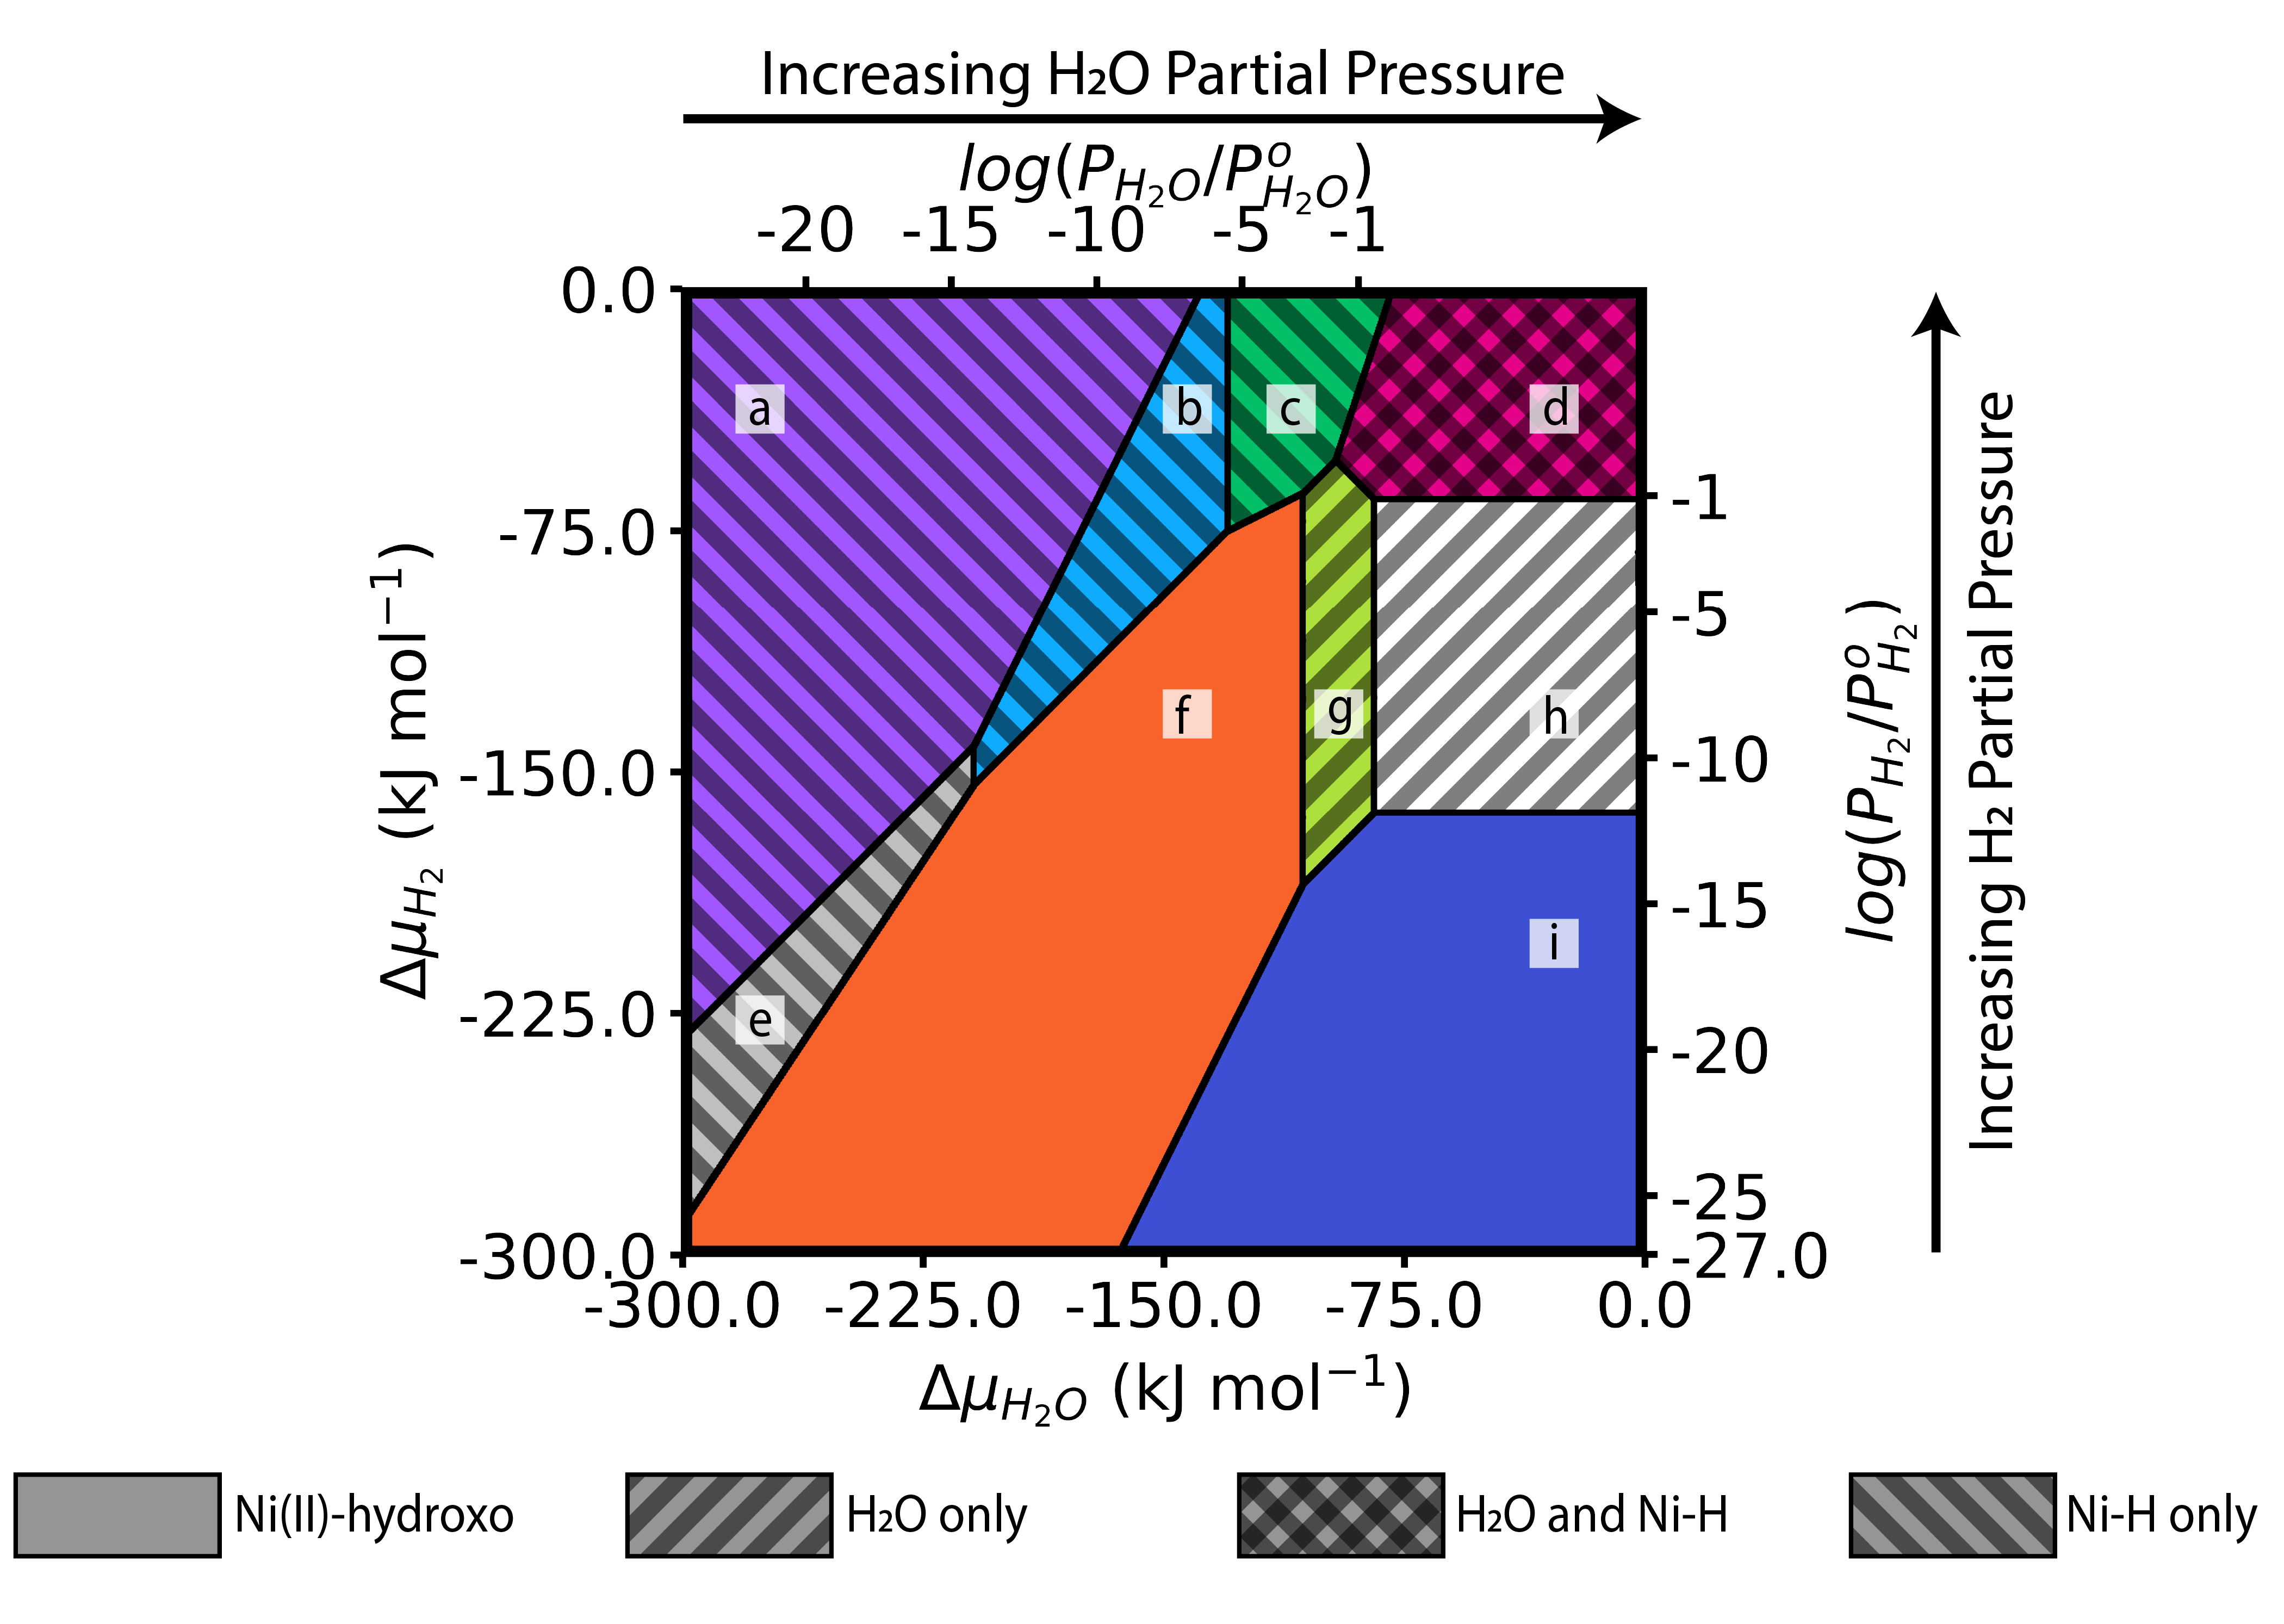
\includegraphics[width=0.95\textwidth]{zi-images/01-Ni-Graphics/2020-08-31-Phase-Diagram-V02.png}
    \caption{Phase diagram generate by \textit{ab initio} thermodynamic analysis that captures the structural stability of a Ni(II) supported metal complex in NU-1000 at \SI{200}{\celsius}. The starting structure is the \ce{Ni4(OH)6} complex. The composition and morphology of the Ni(II) complex changes depending on the \ce{H2} and \ce{H2O} partial pressures, which produces new structural features, such as physisorbed \ce{H2O} and metal hydride structures.}
    \label{fig:phasediagramNi4}
\end{figure}

Figure \ref{fig:phasediagramNi4} shows the stability of the \ce{Ni4(OH)6} metal complex under different hydrogenation conditions. As the partial pressure of \ce{H2} increase (a more positive chemical potential) under ambient conditions, the \ce{OH}-ligands within the \ce{Ni4(OH)6} metal complex are converted into physisorbed \ce{H2O} through the dissociative adsorption of \ce{H2} onto the cluster. Increasing the gas phase \ce{H2} partial pressure, increases the driving force for dissociative adsorption. However, if the partial pressure of \ce{H2O} in the gas phase is too large, the desorption of weakly bound \ce{H2O} molecules is prevented (as shown in Figures \ref{fig:phasediagramNi4} and \ref{fig:structurediagramNi4}). Additionally, \textit{ab initio} thermodynamic analysis suggests that at high enough partial pressure of both \ce{H2O} and \ce{H2} that the cluster can exhibit both physisorbed waters and metal hydride structures.
 

%At sufficient gas phase \ce{H2} partial pressures (e.g.\ log $\frac{P_{\ce{H2}}}{P^{o}_{\ce{H2}}}=-1$ at \SI{200}{\celsius}), the cluster exhibits dynamic structural changes in both morphology and composition. The changes show the breakdown of the Ni(II) metal complex. Specifically, the the \ce{OH}-ligands are systematically replaced by \ce{H} atoms that are forming metal hydride species. The replacement of these \ce{OH}-ligands is clearly demonstrated in Figure \ref{fig:structurediagramNi4}. These structural changes are further illustrated by the reduction in the oxidation state of \ce{Ni} and the decreasing distance between \ce{Ni} atoms (Table \ref{tbl:Ni4oxidationstates}). 

\begin{table}
  \setlength\tabcolsep{8pt}
  \caption{Nickel Formal Charge and \ce{Ni-Ni} Bond Distances.}
  \label{tbl:Ni4oxidationstates}
  \begin{tabular}{lccc}
    \hline
        Structure  &  \thead{\ce{Ni} Formal \\ Charge\textsuperscript{\emph{a}}} &    \thead{Potential \ce{Ni} \\ Oxidation State} & \thead{\ce{Ni-Ni} \\ Distance (A)} \\
    \hline 
    a) \ce{(NiH2Ni)(NiNi)}             & 1             & \ce{Ni(0)}, \ce{Ni(I)}, \ce{Ni(II)}, \ce{Ni(II)}     & 2.23, 2.42 \\   
    b) \ce{(Ni3H2)(Ni)(OH)2}           & $\frac{3}{2}$ & \ce{Ni(I)}, \ce{Ni(I)}, \ce{Ni(II)}, \ce{Ni(II)}     & 2.21, 2.54 \\ 
    c) \ce{(NiH)(Ni3H)(OH)2 * 1H2O}    & $\frac{3}{2}$ & \ce{Ni(0)}, \ce{Ni(II)}, \ce{Ni(II)}, \ce{Ni(II)}     & 2.27, 2.31 \\   
    d) \ce{(Ni2)(NiH)2(OH)4 * 2H2O}    & 2             & \ce{Ni(II)}, \ce{Ni(II)}, \ce{Ni(II)}, \ce{Ni(II)}     & 2.72, 3.17 \\     
    e) \ce{(Ni2H)(NiNi)(OH)}           & 1             & \ce{Ni(0)}, \ce{Ni(I)}, \ce{Ni(I)}, \ce{Ni(II)}     & 2.24, 2.50 \\  
    f) \ce{Ni4(OH)4}                   & $\frac{3}{2}$ & \ce{Ni(I)}, \ce{Ni(I)}, \ce{Ni(II)}, \ce{Ni(II)}   & 2.27, 3.06 \\
    g) \ce{Ni4(OH)4 \cdot 1H2O}        & $\frac{3}{2}$ & \ce{Ni(I)}, \ce{Ni(I)}, \ce{Ni(II)}, \ce{Ni(II)}   & 2.29, 2.96 \\
    h) \ce{Ni4(OH)4 \cdot 2H2O}        & $\frac{3}{2}$ & \ce{Ni(I)}, \ce{Ni(I)}, \ce{Ni(II)}, \ce{Ni(II)}   & 2.33, 3.03 \\
    i) \ce{Ni4(OH)6}                   & 2             & \ce{Ni(II)}, \ce{Ni(II)}, \ce{Ni(II)}, \ce{Ni(II)} & 2.81, 3.03 \\
    \hline
  \end{tabular} \\
  \textsuperscript{\emph{a}} Formal Charge given on a per Ni atom basis. \\
\end{table}

%The replacement of structural \ce{OH}-ligands with \ce{H} atoms, the decreasing of \ce{Ni} oxidation state, and the decreasing \ce{Ni-Ni} distances all suggests that under these reducing conditions the \ce{Ni(II)} metal complex is no longer stable. That is, thermodynamically, under these conditions the metal atoms of the supported metal complex are being liberated, suggesting that the formation of \ce{Ni} nanoparticles is favorable in this regime. The \ce{Ni(II)} atoms are reduced to metallic \ce{Ni(0)}, supported by the formation of metallic \ce{Ni} bonds. 

\begin{figure}[H]
    \centering
    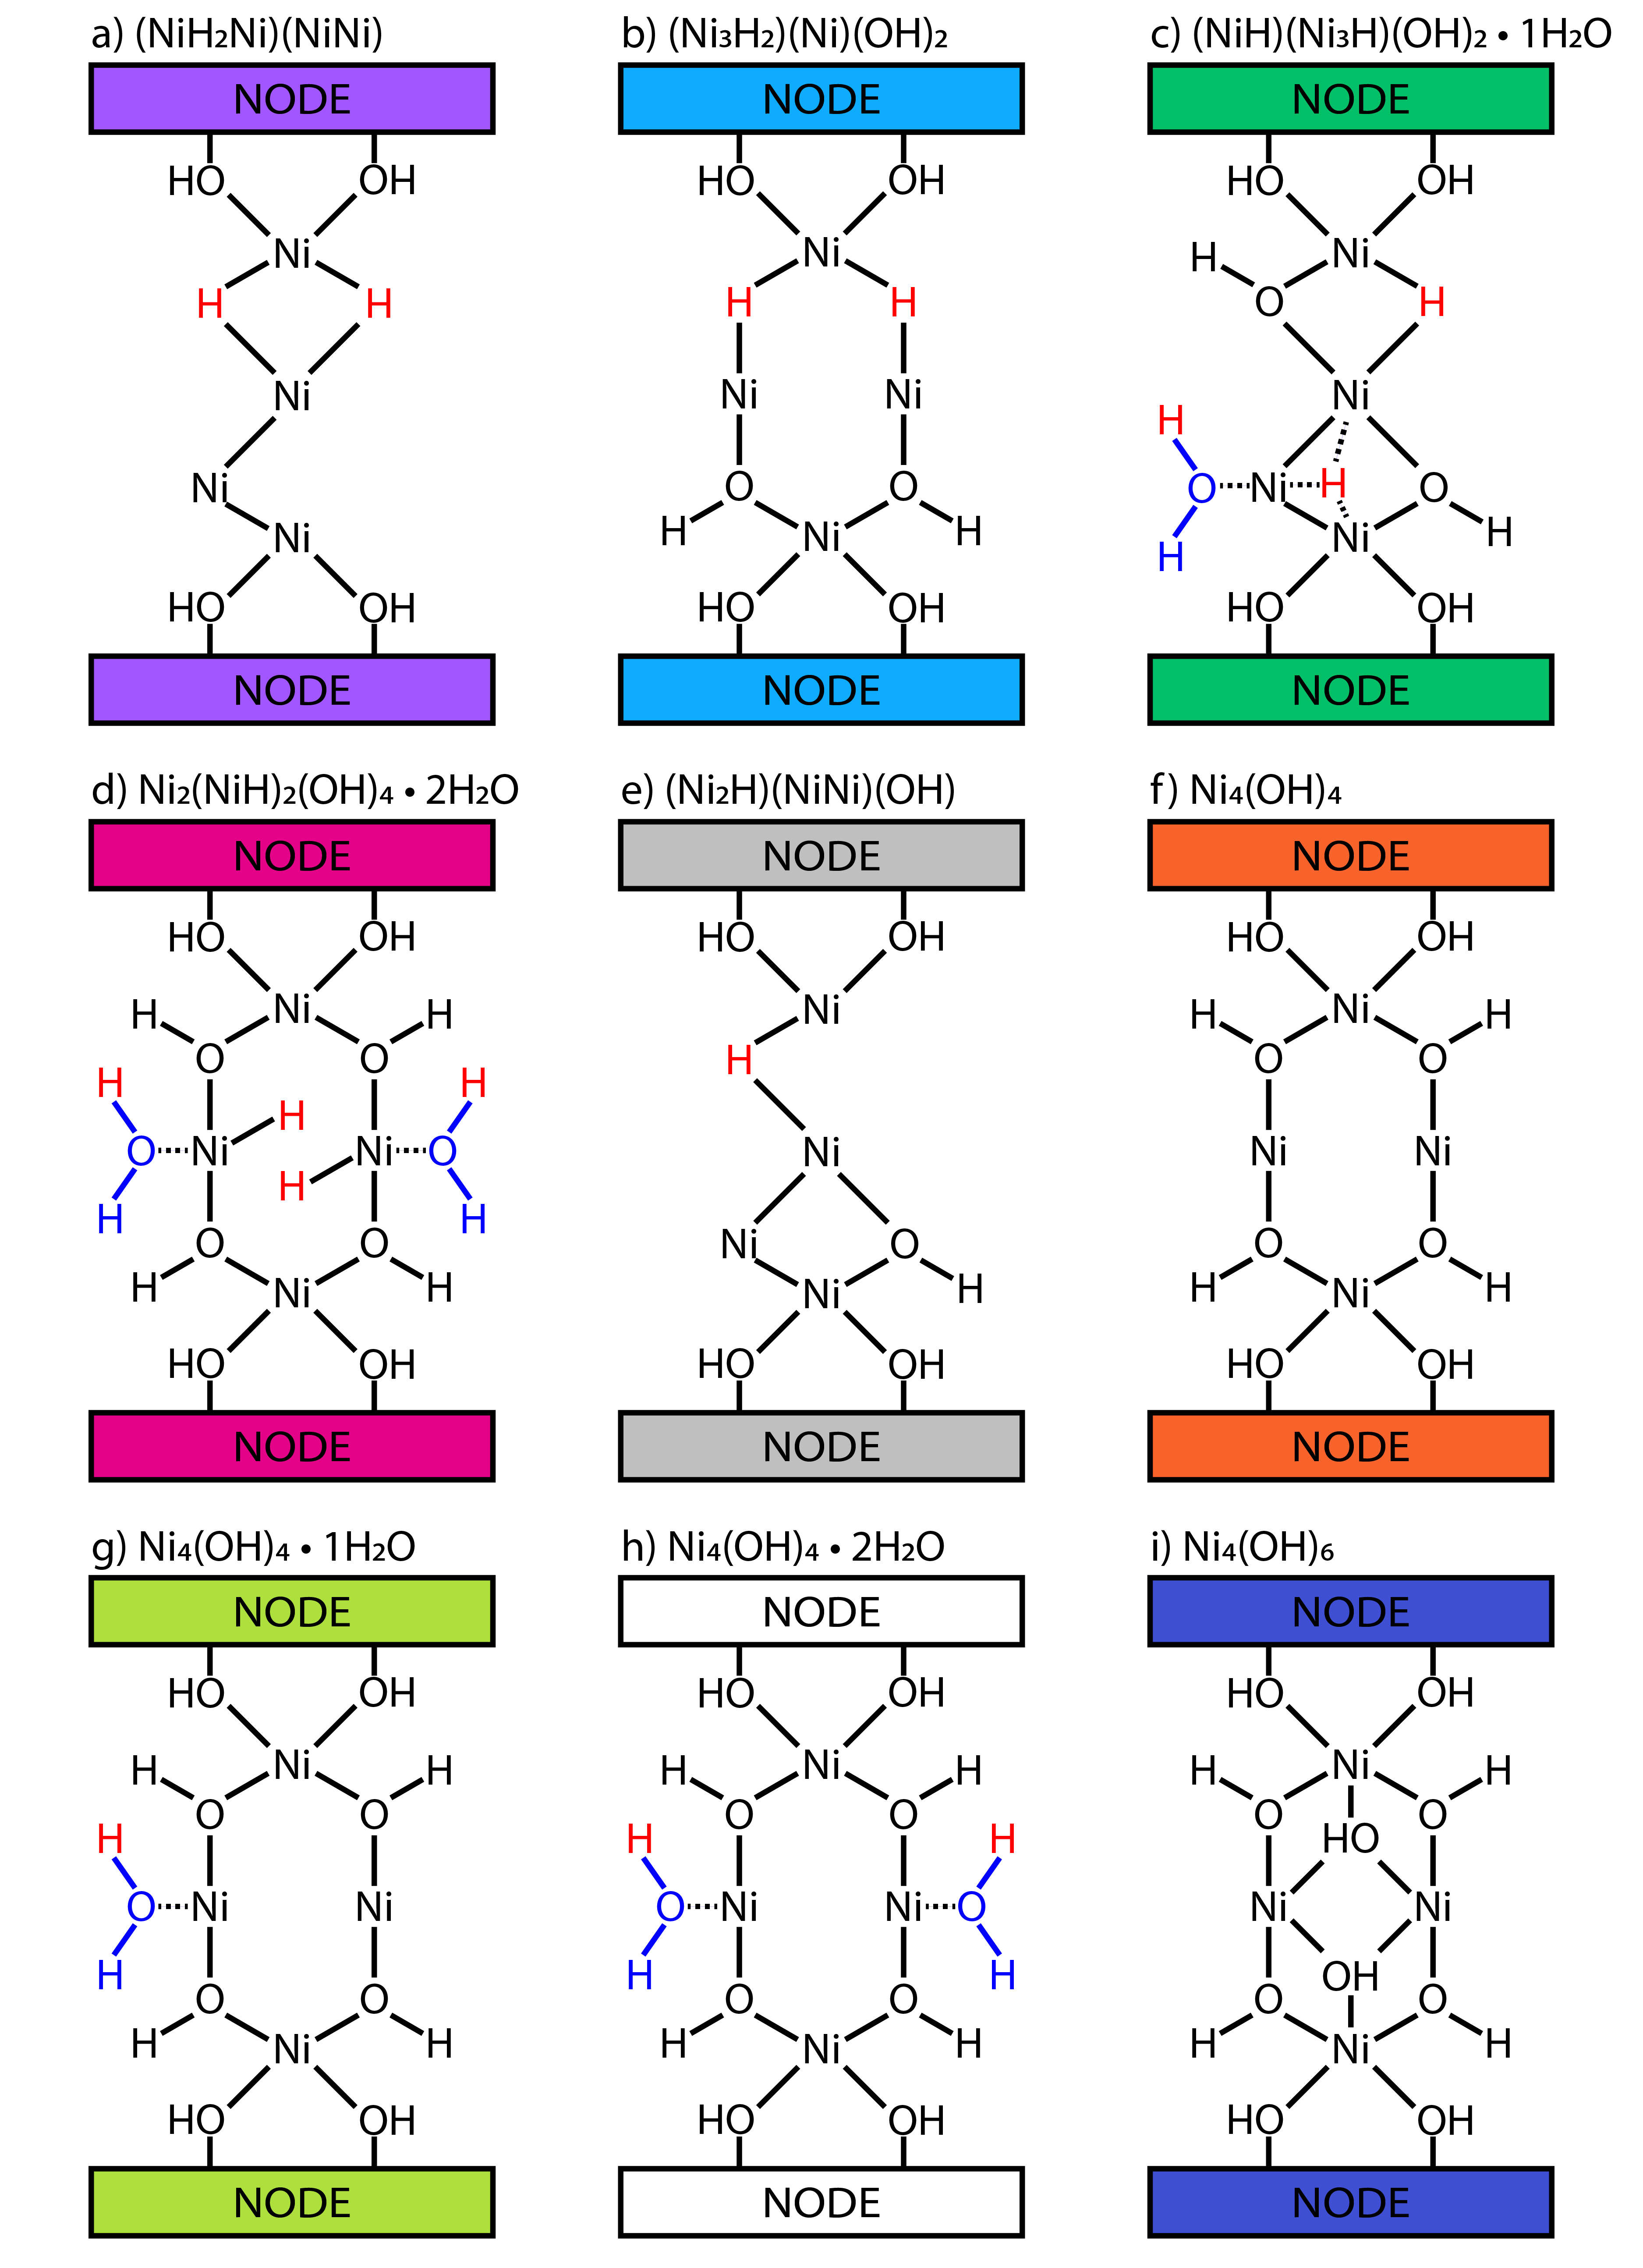
\includegraphics[width=0.85\textwidth]{zi-images/01-Ni-Graphics/2020-08-31-StructureDiagram-V01.png}
    \caption{Schematic representation of the lowest energy structures from the \textit{ab initio} thermodynamic analysis. The node colors scheme correspond to the \ce{Ni(II)} supported metal complex phase diagram (Figure \ref{fig:phasediagramNi4}).}
    \label{fig:structurediagramNi4}
\end{figure}

\begin{itemize}
    \item The \ce{Ni4(OH)6} phase diagram is structurally more diverse than the \ce{Cu3(OH)4} phase diagram (attributed to more metal and \ce{OH}-ligands in the \ce{Ni} metal complex). However, there are similar features as the \ce{Cu3(OH)4 }(\ref{fig:phasediagramCu3}). Both demonstrate metal hydrides, and physisorbed \ce{H2O}.
    \item The presence of \ce{H2O} in the gas phase has a strong influence over the structurally stability. For example, at \ce{H2} partial pressure of ~ $10^-1$ bar, the reduction of the cluster is illustrated going from \ce{Ni2(NiH)2(OH)4} to \ce{(NiH2Ni)(NiNi)}. At higher \ce{H2O} partial pressure, the cluster is more likely to exist as a combination of \ce{Ni-H} and physisorbed \ce{H2O}. As the partial pressure of \ce{H2O} decreases, the formed physisorbed \ce{H2O} is removed. Overall, if the cluster is exposed to a sufficient \ce{H2} gas the cluster is reduced. 
    \item The main structures to focus on are the structures that demonstrate the \ce{Ni} reduction from \ce{Ni(II)} to \ce{Ni(0)}. These structures reveal the presence of metallic \ce{Ni} bonds (the more mobile species).
\end{itemize}

%%%%%%%%%%%%%%%%%%%%%%%%%%%%%%%%%%%%%%%%%%%%%%%%%%%%%%%%%%%%%%%%%%%%%
%% Discussion
%%%%%%%%%%%%%%%%%%%%%%%%%%%%%%%%%%%%%%%%%%%%%%%%%%%%%%%%%%%%%%%%%%%%
\newpage
\subsection{Discussion}
\begin{itemize}
    \item The structural characteristics of the supported metal complexes are dependent on the reaction conditions.
    \begin{itemize}
        \item In the presence of a reducing agent (\ce{H2}), the hydroxo-ligands of the supported metal complexes are removed (as \ce{H2O}). As previously suggested, we show computationally that \ce{H2} is important in breaking the bonds between the metal clusters and the NU-1000 nodes. We provide the thermodynamic landscape for these transformations.
        \item Our findings show similar structural features and suggest that in an \ce{H2} reducing environment these supported metal complexes containing \ce{OH}-ligands are not stable.  
        \item At present, our modeling efforts demonstrate the formation of the more mobile \ce{M(0)} species. The breakdown of the supported metal complex (removal of \ce{OH}-ligands within the cluster) reduces the metal atoms, thereby generating the mobile \ce{M(0)} species.
    \end{itemize}
    \item A key question that still remains is whether these reduced supported metal complexes still exist as a combination of NPs and multinuclear metal active sites or mononuclear active sites (single-sites) above \SI{200}{Celsius}.
    \begin{itemize}
        \item \citeauthor{Halder2020} determined that in an \ce{H2} environment the \ce{Cu3(OH)4} supported metal complexes showed large \ce{Cu} NP formation. These particles were ~6.0 nm in diameter, which is larger than the ~3.0 nm diameter hexagonal pore in NU-1000. Therefore, for \ce{Cu}-NU-1000 we know that these NPs grow, and we show using our modeling that for \ce{Ni} we expect \ce{Ni} NPs to grow as well. 
        \item Our present results support the experimental findings of \citeauthor{Halder2020} that reduced metal atoms are generated. However, we extend the findings further and hypothesize that some of the single-site metal atoms remain intact. Not all of the metal atoms are reduced to \ce{M(0)}; the metal atoms attached to the \ce{OH}-ligands of the node remain. 
        \item There are a few more additional calculations to be computed to test our theory (and these calculations are currently being performed). The calculations contain two single-site models (with and without the \ce{M-H} species). The metal atoms removed from the system will be accounted for as nanoclusters.
    \end{itemize}
\end{itemize}
We have the following list of questions:
\begin{itemize}
    \item Experimentally, there is a different in the protocols to generate the single-site and the clusters in NU-1000? Experimentally, you can differentiate between the two different catalysts in NU-1000? 
    \item When looking at the Cu-NU-1000 discussion, did you ever remove the Cu-NPs and determine whether the framework that was left behind was catalytically active? We wonder whether or not all the metal atoms are becoming the mobile \ce{M(0)} species. 
    \item The hexagonal pore returned to its original ~34 A value. How does the value of the pore compare when there are single-site metal atoms attached to the node? 
\end{itemize}

%\subsection{References}

%The class makes various changes to the way that references are
%handled.  The class loads \textsf{natbib}, and also the
%appropriate bibliography style.  References can be made using
%the normal method; the citation should be placed before any
%punctuation, as the class will move it if using a superscript
%citation style
%\cite{Mena2000,Abernethy2003,Friedman-Hill2003,EuropeanCommission2008}.
%The use of \textsf{natbib} allows the use of the various citation
%commands of that package: \citeauthor{Abernethy2003} have shown
%something, in \citeyear{Cotton1999}, or as given by
%Ref.~\citenum{Mena2000}.  Long lists of authors will be
%automatically truncated in most article formats, but not in
%supplementary information or reviews \cite{Pople2003}. If you
%encounter problems with the citation macros, please check that
%your copy of \textsf{natbib} is up to date. The demonstration
%database file \texttt{achemso-demo.bib} shows how to complete
%entries correctly. Notice that ``\latin{et al.}'' is auto-formatted
%using the \texttt{\textbackslash latin} command.

%Multiple citations to be combined into a list can be %given as
%a single citation.  This uses the \textsf{mciteplus} %package
%\cite{Johnson1972,*Arduengo1992,*Eisenstein2005,*Arduengo%1994}.
%Citations other than the first of the list should be %indicated
%with a star. If the \textsf{mciteplus} package is not %installed,
%the standard bibliography tools will still work but %starred
%references will be ignored. Individual references can be %referred
%to using \texttt{\textbackslash mciteSubRef}:
%``ref.~\mciteSubRef{Eisenstein2005}''.

%The class also handles notes to be added to the bibliography.  These
%should be given in place in the document \bibnote{This is a note.
%The text will be moved the the references section.  The title of the
%section will change to ``Notes and References''.}.  As with
%citations, the text should be placed before punctuation.  A note is
%also generated if a citation has an optional note.  This assumes that
%the whole work has already been cited: odd numbering will result if
%this is not the case \cite[p.~1]{Cotton1999}.

%%%%%%%%%%%%%%%%%%%%%%%%%%%%%%%%%%%%%%%%%%%%%%%%%%%%%%%%%%%%%%%%%%%%%
%% The "Acknowledgement" section can be given in all manuscript
%% classes.  This should be given within the "acknowledgement"
%% environment, which will make the correct section or running title.
%%%%%%%%%%%%%%%%%%%%%%%%%%%%%%%%%%%%%%%%%%%%%%%%%%%%%%%%%%%%%%%%%%%%%
%\begin{acknowledgement}
%
%\hl{authors would like to thank \ldots''.
%
%The author thanks Mats Dahlgren for version one of \textsf{achemso},
%and Donald Arseneau for the code taken from \textsf{cite} to move
%citations after punctuation. Many users have provided feedback on the
%class, which is reflected in all of the different demonstrations
%shown in this document.}
%
%\end{acknowledgement}

%%%%%%%%%%%%%%%%%%%%%%%%%%%%%%%%%%%%%%%%%%%%%%%%%%%%%%%%%%%%%%%%%%%%%
%% The same is true for Supporting Information, which should use the
%% suppinfo environment.
%%%%%%%%%%%%%%%%%%%%%%%%%%%%%%%%%%%%%%%%%%%%%%%%%%%%%%%%%%%%%%%%%%%%%
%\begin{suppinfo}
%
%\hl{This will usually read something like: ``Experimental procedures and
%characterization data for all new compounds. The class will
%automatically add a sentence pointing to the information on-line:}
%
%\end{suppinfo}

%%%%%%%%%%%%%%%%%%%%%%%%%%%%%%%%%%%%%%%%%%%%%%%%%%%%%%%%%%%%%%%%%%%%%
%% The appropriate \bibliography command should be placed here.
%% Notice that the class file automatically sets \bibliographystyle
%% and also names the section correctly.
%%%%%%%%%%%%%%%%%%%%%%%%%%%%%%%%%%%%%%%%%%%%%%%%%%%%%%%%%%%%%%%%%%%%%
\newpage
\bibliography{achemso-demo}

\end{document}